
% --------------------------------------------------------------------
% This is a simple Beamer document that uses beamerthemesigma.sty
% Reading the comments should help you create a presentation even if
% you've never used Beamer before.
% --------------------------------------------------------------------
% Set our document class to Beamer
\documentclass[aspectratio=169]{beamer}

% Some packages for nice font encodings in the final PDF
\usepackage[utf8]{inputenc}
\usepackage[T1]{fontenc}

% From Jeff E
\usepackage{algo}

\usepackage{sigmastyle}

% To insert images
\usepackage{graphicx}

% Useful packages from the AMS
\usepackage{amsmath,amssymb,amsthm}

% for parse tree
\usepackage{forest}

% Package for code highlighting
\usepackage{minted}
\setminted{linenos=true, breaklines=true, breakanywhere=true}
% \usemintedstyle{monokai}
% \usemintedstyle{native}

% Set a title
\title{Parsing}

% The subtitle is generally where I'd expect you to put the week
% number, thus:
\subtitle{Week 5}
% \texorpdfstring to remove compilation warnings if you have math here

% Whoever worked on the presentation:
\author{Hassam}

% A date, if you'd like.
\date{}

% An institute name, if you're so inclined
% \institute{University of Illinois Urbana-Champaign}

% Use the SIGma theme for this Beamer presentation
\usetheme{sigma}
% --------------------------------------------------------------------
% Begin document
\begin{document}

% Beamer calls each slide a "frame", defined within the environment:
% \begin{frame}
%   <frame content here>
% \end{frame}

% This frame is just the title.
\begin{frame}
\titlepage
\end{frame}

% A frame with the table of contents.
% This frame's title is "Outline".
\begin{frame}{Outline}
  \tableofcontents
\end{frame}

% % The frame title is a flag.
% \begin{frame}{Updates!}
%   % Let's put some real content in this frame:
%   \pause
%   \begin{itemize}
%     \item We want feedback
%   \end{itemize}
% \end{frame}

\section{Compilers}
\frame{\sectionpage}

\begin{frame}{C to executable?}
    How do you go from "code" to something the computer understands? \pause 
    \begin{itemize}
        \item What does the computer even understand? \pause 
        \item What is code? 
    \end{itemize}
\end{frame}

\begin{frame}{Assembly}
    @nebu addressed this two weeks ago, but let's review.
\end{frame}

\begin{frame}{}
    \begin{center}
        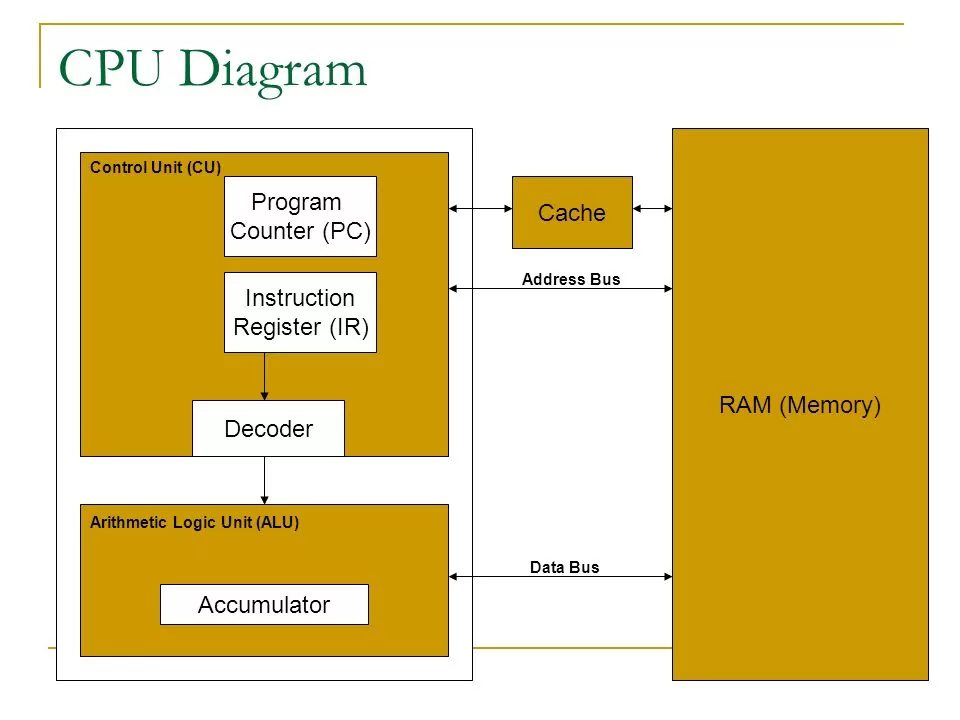
\includegraphics[width=\textwidth]{cpu.png}
    \end{center}
\end{frame}

\begin{frame}{}
    \begin{center}
        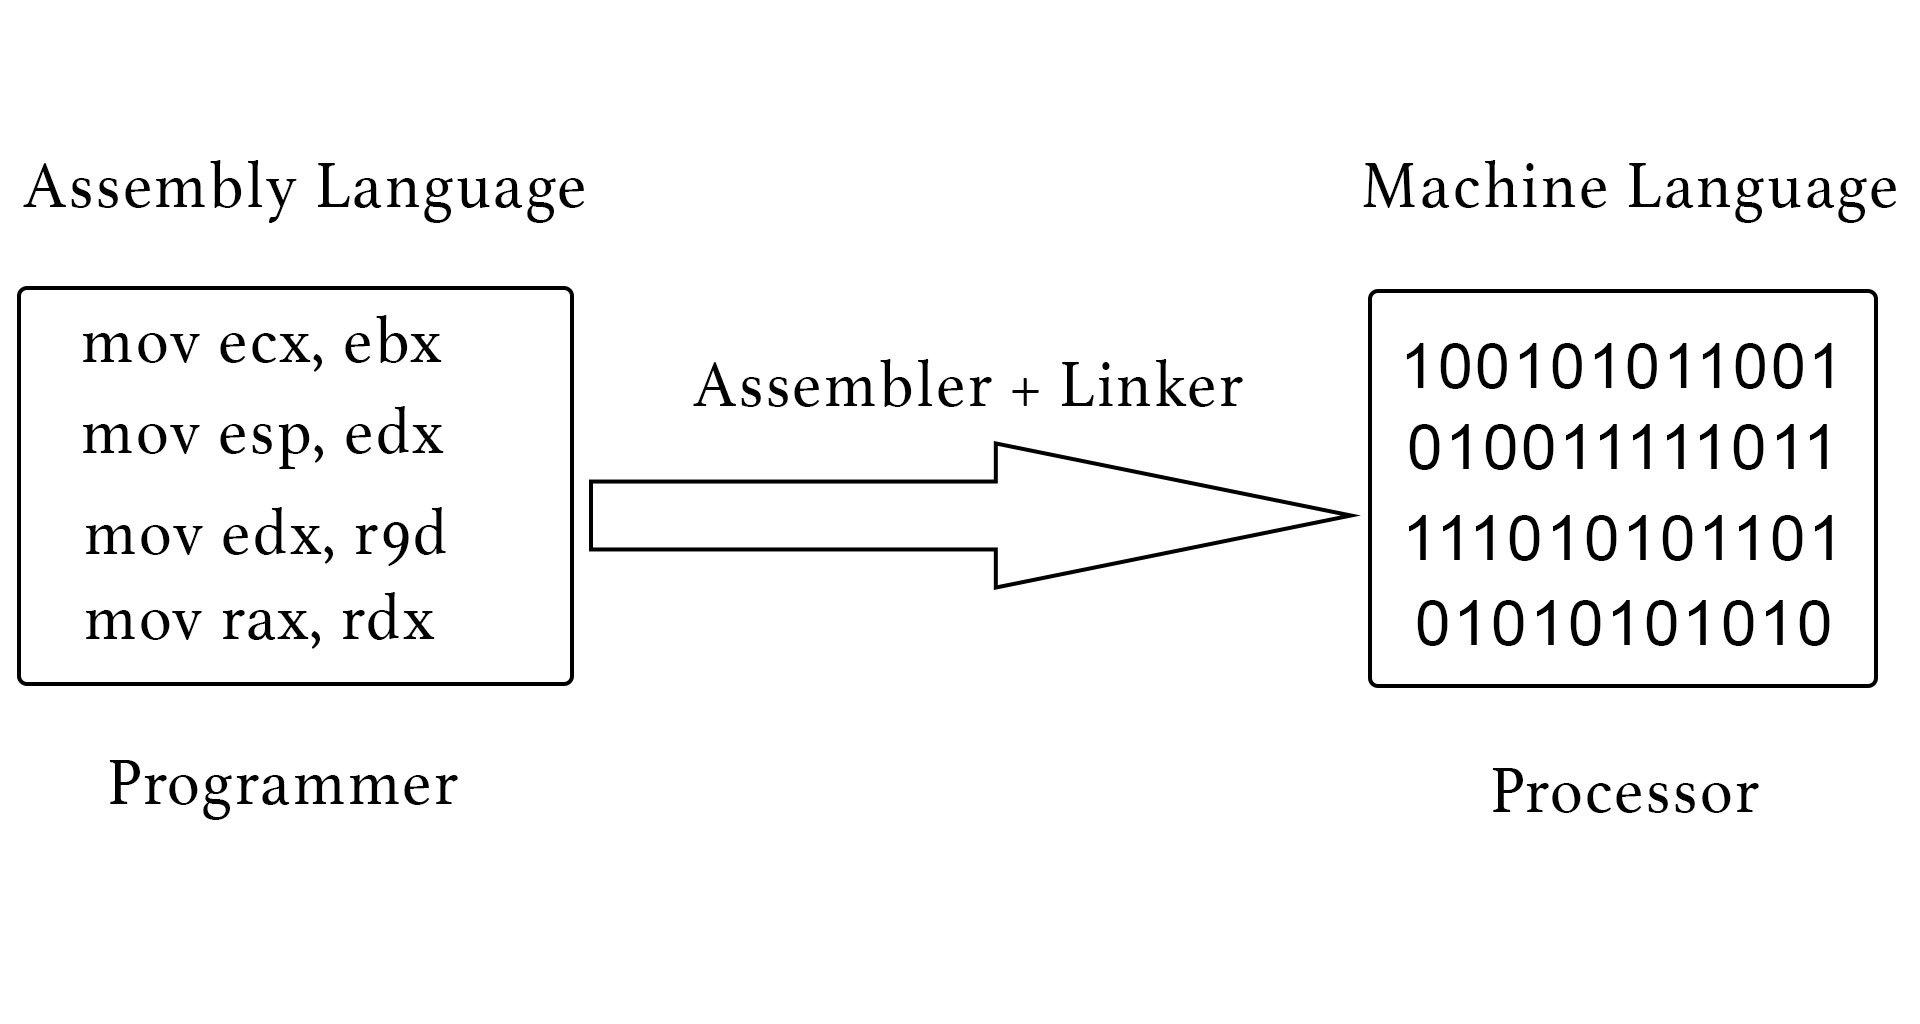
\includegraphics[width=\textwidth]{assembly.png}
    \end{center}
\end{frame}

\begin{frame}[fragile]{Code?}
\begin{minted}{c}
int main(int argc, char** argv) {
    puts("Hello, World!");
    return 0;
}
\end{minted}
\end{frame}
\begin{frame}[fragile]{Code?}
\begin{minted}{python}
def main():
    print("Hello, world!")
\end{minted}
\end{frame}

\begin{frame}{What are the steps in between?}
    \begin{tikzpicture}[
box/.style={draw,rectangle, rounded corners, fill=yellow!20, minimum width=3cm, minimum height=1cm},
a/.style={thick,->,>=stealth}
    ]
        \node[box] (lexer) at (-2, 0) {Lexer};
        \only<1>{\node[inner sep=0pt] (token) at (-2, -2) {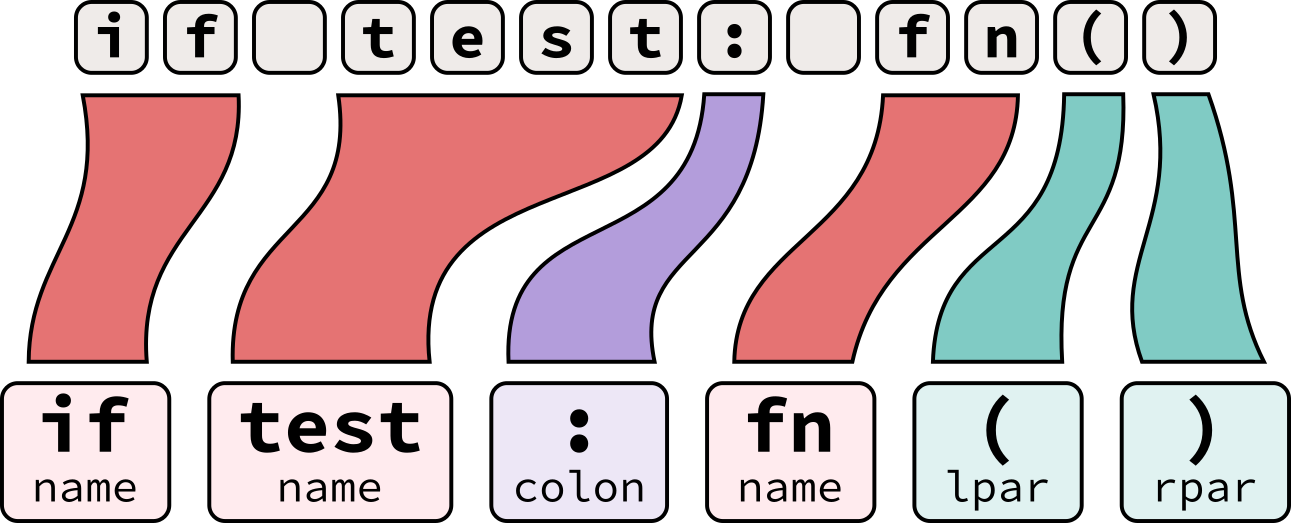
\includegraphics[width=0.4\textwidth]{tokenization.png}}};
        \onslide<2->{\node[box] (parser) at (2, 0) {Parser}; \draw[a] (lexer) -- (parser);};
        \only<2>{\node[inner sep=0pt] (tree) at (2, -3) {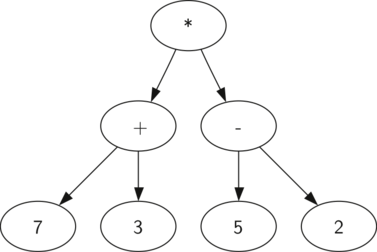
\includegraphics[width=0.4\textwidth]{parsetree.png}}};
        \onslide<3->{\node[box] (sa) at (2, -2) {Semantic Analysis}; \draw[a] (parser) -- (sa);};
        \only<3>{\node[align=center] (notes) at (2, -3.5) {Syntax Errors \\ Type Checking \\ Lifetime Analysis}};
        \onslide<4->{\node[box] (cg) at (6, -2) {Codegen}; \draw[a] (sa) -- (cg);};
        \only<4>{\node[align=center] (notes) at (6, -3.5) {Assembly! \\ Optimizations}};
    \end{tikzpicture}
\end{frame}

\begin{frame}{}
      \begin{center}
    {\color{sigma@mainblue} \LARGE Questions?}
  \end{center}
\end{frame}

% Start a section: *sections* (subsections, etc.) are what show up in the TOC.
\section{Parsing}
% Section pages can be printed thus:
\frame{\sectionpage}
% There's a way to automate this, see:
% https://tex.stackexchange.com/questions/178800/creating-sections-each-with-title-pages-in-beamers-slides/178803

\begin{frame}{Remember CFGs?}
    \begin{itemize}
        \item So far, we have been using CFGs without any reason. 
        \item Soon, we'll use them to prove properties of computation! \pause
        \item But, sometimes you just want to specify a grammar and parse it, CFGs are useful here too! 
        \item CFGs are ugly though, and we're leaving the world of theory, so we have something better. 
    \end{itemize}
\end{frame}

\begin{frame}[fragile]{Extended Backus–Naur form}
    \begin{minted}{c}
file = line { line } <EOF>.
line = [ assignment | print | reset ] <NL>.
assignment = var ":=" expression.
print = "PRINT" var.
reset = "RESET".
expression = term { addop term }.
term = factor { mulop factor }.
factor = "(" expression ")" | var | number.
addop = "+" | "-".
mulop = "*". 
var = letter { letter | digit }.
number = [ "-" ] digit { digit }.
letter = ('A'-'Z') | ('a'-'z').
digit = ('0'-'9').
    \end{minted}
\end{frame}

\begin{frame}{Parse Tree}
    \begin{forest}
    [file
        [line
          [assignment
            [var ["x"]]
            ["\text{=}"]
            [expression
              [term [... [12]]]
              [addop ["+"]]
              [term [... [15]]]
            ]
          ]
        ]
        [line
          [print
            ["PRINT"]
            [var ["x"]]
          ]
        ]
    ]
    \end{forest}
\end{frame}

\begin{frame}[fragile]{Parse Tree}
\begin{minted}{python}
x = 12 + 15
PRINT x
\end{minted}
\end{frame}

\begin{frame}{So, PDAs?}
    \begin{itemize}
        \item This "language" is representable by a CFG, so should we use a PDA to parse it? \pause
        \item Let's not. 
    \end{itemize}
\end{frame}

\begin{frame}{LL Parsing}
    \begin{itemize}
        \item Reading \textbf{L}eft to right, performing a \textbf{L}eftmost processing.
        \item Formally, this type of parser is equivalent to a deterministic pushdown automata. But, much easier to write.
        \item Requires our grammar to follow some rules, but all grammars (parseable by DPDAs) can be (annoyingly) converted to do so. 
    \end{itemize}
\end{frame}

\begin{frame}[fragile]{Easy to write?}
    So easy to write: 
\begin{minted}{python}
start = F | '(' start '+' F ')'
F = 'a'
\end{minted}
This parses expressions of the form: (a + a), ((a + a) + a), etc. 
\end{frame}

\begin{frame}[fragile]{How do we code this?}
\begin{columns}[T]
    \begin{column}{0.6\textwidth}
        \begin{minted}{haskell}
parseF 'a':xs = F, xs
parseF [] = error

parseS '(':xs = {
    S1, '+':restS = parseS(xs)
    F, ')':rest = parseF(restS)
    return (S (S1, F)), rest
}
parseS x = {
    F, rest = parseF(x)
    return S(F), rest
}
parseS [] = error
\end{minted}
    \end{column}
    \begin{column}{0.4\textwidth}
        \begin{minted}{python}
start = F 
  | '(' start '+' F ')'
F = 'a'
\end{minted}
    \end{column}
\end{columns}

\end{frame}

\begin{frame}{What goes wrong?}
    \begin{itemize}
        \item Our code from before is valid and generalizable, but it makes some assumptions. \pause 
        \item It assumes that there is no "left recursion" \pause
        \item It assumes that there are no common prefixes \pause
        \item It assumes that you can look one character ahead and determine what to do next. This is formally known as LL(1). \pause 
        \item It assumes there's no ambiguity. \pause 
    \end{itemize}
    Which of these can we fix? 
\end{frame}

\begin{frame}[fragile]{Ambiguity?}
\begin{minted}{c++}
void func() {
    a < b , c > d;
}
\end{minted}
\pause
Is this a template instantiation? Or are we using \mintinline{c++}{operator<} and \mintinline{c++}{operator>} on two variables? \\ \pause 
It's both. 
\end{frame}

\begin{frame}{Fixing bad grammars}
    It turns out, we can fix them all, except for the last one. We need a more powerful tool for ambiguity.
    \begin{itemize}
        \item It is possible to rewrite anything left-recursive to be non-left-recursive.
        \item Removing common prefixes is called "left factoring". 
        \item We can change from an LL(1) parser to an LL(k) parser, and "look ahead" k steps. This becomes messier and messier the further we look ahead though. 
    \end{itemize}

    Nearly every mainstream programming language is LL(1). They are convenient to parse, and even more convenient to write. 
\end{frame}

\begin{frame}[fragile]{Fixing left recursion}
\begin{minted}{c}
start = start '+' | 'i'
\end{minted}
This parses i+++++, and onwards. How do we get rid of the left recursion? 
\pause 

The general strategy is:
\begin{itemize}
    \item \mintinline{c}{S = 'x'} becomes \mintinline{c}{S = 'x'S_new}
    \item \mintinline{c}{S = S'x'} becomes \mintinline{c}{S_new = 'x'S_new}
    \item Add \mintinline{c}{S_new =} $\epsilon$
\end{itemize}
\pause 
\begin{minted}[escapeinside=;;]{c}
start = 'i' start_new
start_new = '+'start_new | ;$\epsilon$;
\end{minted}
\end{frame}

\begin{frame}[fragile]{Fixing common prefixes}
\begin{minted}{c}
start = 'a' B | 'a' 'd'
B = 'c'
\end{minted} 
\pause 
Becomes:

\begin{minted}{c}
start = 'a' D
D = B | 'd'
B = 'c'
\end{minted} 

\end{frame}

\begin{frame}{Solving Ambiguity}
    Remember our CFG from last week? 
    {
    \Large
    \begin{align*}
        S ~\to~ \varepsilon ~&|~ S\texttt{a}\texttt{b} ~|~ \texttt{a}S\texttt{b} ~|~ \texttt{a}S\texttt{b}S  \\
          ~&|~ S\texttt{b}\texttt{a} ~|~ \texttt{b}S\texttt{a} ~|~ \texttt{b}S\texttt{a}S
    \end{align*}
    }
We can try to fix the left recursion and the common prefixes, but we'll get stuck in an infinite loop. This grammar is "ambiguous", we would need to look ahead infinitely many steps to parse it. We need non-determinism to parse this. 
\end{frame}

\begin{frame}[fragile]{Backtracking to the rescue?}
\begin{minted}[fontsize=\small]{python}
def parseS(inp):
    if inp == '': return S(), '' 
    try:
        s, rest = parseS(inp)
        if rest[0] == 'a':
            assert rest[1] == 'b'
            return S(s, 'a', 'b'), rest[2:]
        elif rest[0] == 'b':
            assert rest[1] == 'a'
            return S(s, 'b', 'a'), rest[2:]
        else:
            assert False
    except Exception:
        assert inp[0] == 'a'
        try: 
            s, rest = parseS(inp)
            ...
\end{minted}
\end{frame}

\begin{frame}{Yikes}
     This is messy, and it's slow! Try finishing it by yourself.

    Most modern compilers for non-LL(1) languages [C and C++ :( ] use handwritten backtracking parsers like this one. 
\end{frame}

\begin{frame}{Writing parsers for fun and profit}
    Writing parsers is actually very fun! I have had four interviews this semester that required writing a custom parser. 
    \begin{itemize}
        \item Try writing parsers for some of the simple examples we discussed today in your favorite language. 
        \item Go meta. Write a "parser compiler" that takes some basic version of EBNF and turns it into code that runs a parser. 
        \item So much more to explore. LR(k), LALR(k), etc.
        \item Parsing is "solved", more interesting problems in compilers now.  
    \end{itemize}
\end{frame}

\font\eightss=cmssq8
\font\eightssi=cmssqi8
\newcommand\quoteAuthorDate[3]{\begingroup
  \baselineskip 10pt
  \parfillskip 0pt
  \interlinepenalty 10000 % not needed in example
  \leftskip 0pt plus 40pc minus \parindent
  \let\rm=\eightss
  \let\sl=\eightssi
  \everypar{\sl}#1\par
  \nobreak\smallskip
  \noindent\rm--- #2\unskip\enspace(#3)\par
  \endgroup}

\begin{frame}{Goodbye}
    \centering
    \quoteAuthorDate{Any sufficiently complicated C or Fortran program contains an ad hoc, informally-specified, bug-ridden, slow implementation of half of Common Lisp.}{Greenspun's tenth rule of programming}{1993}
\end{frame}


\end{document}